\clearpage

\section{等待CSMA的提出及分析}
第三章所构建的等待 ALOHA 协议为离散等长时隙下的 AoI 优化提供了基础理论框架。然而，在实际的物联网部署中，设备往往具备载波侦听能力。本章将进一步把等待机制拓展至更复杂、更贴近实际物理层的 CSMA 环境中。

\subsection{系统模型}
我们考虑一个包含一个 AP 和 $N$ 个设备的无线网络，各个设备采纳载波侦听的方式接入网络并进行数据传输，如 IEEE 802.11 协议，如图\ref{fig:cp4_system_model}所示。
\begin{figure}[h]
\centering
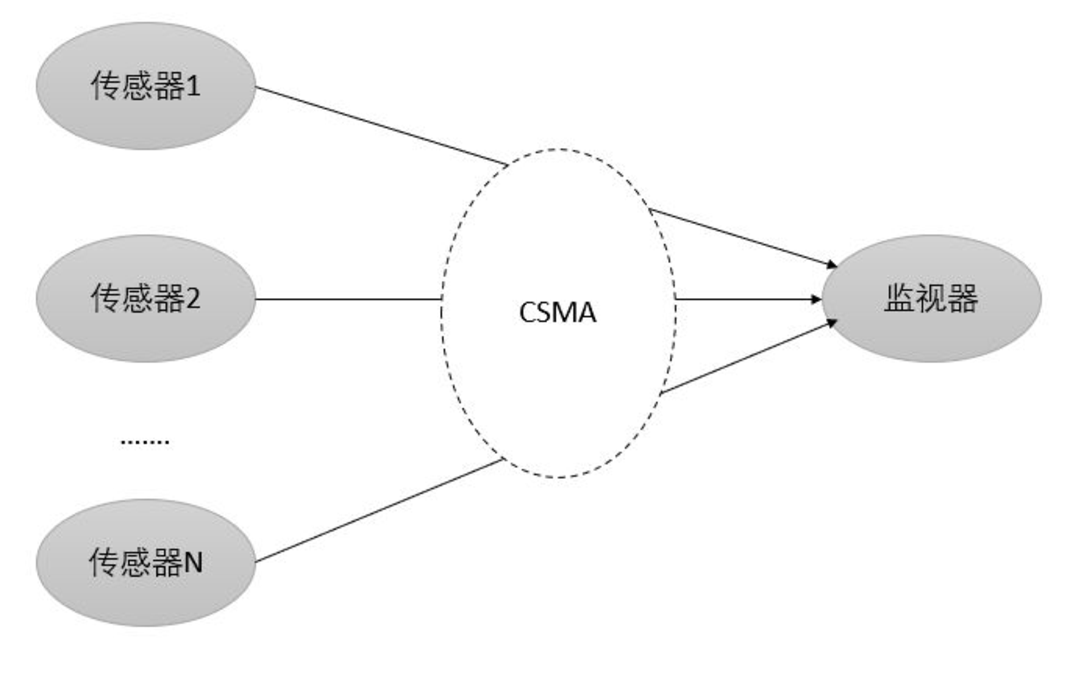
\includegraphics[width=0.8\textwidth]{figure/cp4/系统模型.pdf}
\caption{系统模型图}
\label{fig:cp4_system_model}
\end{figure}

在CSMA中，每个设备在每次传输前会随机生成一个退避计时器。为了降低碰撞概率，每个设备只有在退避计时器归零时才能传输数据包以更新其最新状态。具体而言，每当无线信道在一个微时隙内被感知为空闲时，退避计时器将减少1，而当无线信道被感知为忙碌时，退避计时器将暂停，直到介质再次在一个 DCF 帧间隔（Distributed Inter-frame Spacing，DIFS）内被感知为空闲后再减1，如图\ref{fig:cp4_csma_and_system_slot}所示。
\begin{figure}[h]
\centering
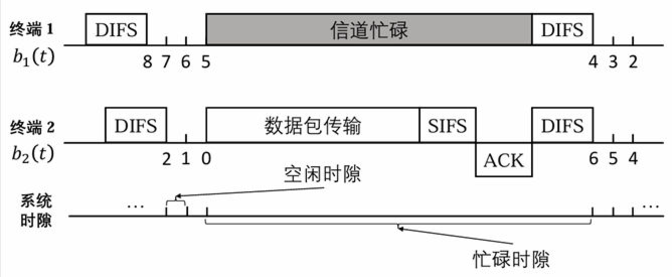
\includegraphics[width=0.8\textwidth]{figure/cp4/CSMA机制与系统时隙的图示.pdf}
\caption{CSMA机制与系统时隙的图示}
\label{fig:cp4_csma_and_system_slot}
\end{figure}

我们将每个系统时隙定义为退避计时器改变之间的间隔。例如，在第 $t$ 个系统时隙开始时，如果第 $i$ 个设备的退避计时器 $b_i(t)$ 不等于0，它将会进行退避，在经过一个系统时隙后退避计时器减少1；此外，如果 $b_i(t)=0$，则第 $i$ 个设备将发送数据包，进而基于发送结果随机生成一个新的退避计时器。由于系统时隙可能为空闲，即无任何设备传输，或忙碌，即至少有一个设备传输，因此它们的持续时间可能不同。我们用归一化后的 $\frac{1}{M}$ 指代每个空闲系统时隙的长度，用1指代每个忙碌系统时隙的长度，即每次数据传输的时长是微时隙的 $M$ 倍，则每个系统时隙的长度 $d(t)$ 可以表示如下：
\begin{equation}
    d(t) = 
\begin{cases} 
\frac{1}{M}, & \text{if } b_i(t) \neq 0, \forall i, \\
1, & \text{if } b_i(t) = 0, \exists i.
\end{cases}
\end{equation}
根据 AoI 的定义，每个设备在每个系统时隙中 AoI 的变化方式如下：
\begin{equation}
    \Delta_t(t + 1) =
\begin{cases}
\Delta_i(t) + \dfrac{1}{M}, & \text{if } b_i(t) \neq 0, \, b_j(t) \neq 0 \, \forall j, \\
1, & \text{if } b_i(t) = 0, \, b_j(t) \neq 0 \, \forall j, \\
\Delta_i(t) + 1, & \text{if } b_j(t) = 0 \, \exists j
\end{cases}
\end{equation}
式中，三种条件分别表示网络中所有设备的退避计数器均为非0，即在该系统时隙中没有任何设备进行传输，因此AoI增加 $\frac{1}{M}$；该设备的退避计数器为0，且网络中其余设备的退避计数器均为非0，则该设备将成功传输，因此AoI降低为1；网络中至少有两个设备退避计数器为0，传输发生碰撞，因此AoI上升1。根据我们所提的系统模型，我们能够绘制出如图\ref{fig:cp4_csma_aoi_evolution}的AoI演化图。
\begin{figure}[h]
\centering

\includegraphics[width=0.8\textwidth]{figure/cp4/AoI变化趋势图.pdf}
\caption{AoI演化趋势图}
\label{fig:cp4_csma_aoi_evolution}
\end{figure}

在mMTC场景中，网络依然面临着与第三章相同的痛点：刚成功传输的设备拥有绝对新鲜的 AoI，短期内连续抢占信道毫无意义；而 AoI 极高、亟需更新的设备却往往因竞争劣势而陷入长期饥饿。因此，我们需要在 CSMA 中引入主动退避机制。我们规定：

\textbf{在每次成功传输后：}该设备根据 $z+\beta \sim \text{unif}(0,w-1)$ 生成新的退避计数器，其中 $z$ 是一个常数等待窗口，用于迫使刚成功更新的设备在接下来的 $z$ 个系统时隙内不参与竞争。这一等待窗口为其他尚未成功传输的设备提供了更多访问信道的机会。类似于现有的 DCF，$\beta \sim \text{unif}(0,w-1)$为在竞争窗口 $w$ 内均匀分布的随机变量，旨在降低碰撞概率。

\textbf{在每次传输失败后：}该设备根据$\beta \sim \text{unif}(0,w-1)$生成新的退避计数器，旨在尽快传输其传感数据包。

根据这个退避机制，我们可以写出每个设备 $i$ 在每个系统时隙的退避计时器变化关系：
\begin{equation}\label{cp4_backoff_counter_evolution}
    b_i(t + 1) =
\begin{cases}
z + \beta, & \text{if } b_i(t) = 0, \, b_j(t) \neq 0 \ \forall j, \\
\beta, & \text{if } b_i(t) = 0, \, b_j(t) = 0 \ \exists j, \\
b_i(t) - 1, & \text{if } b_i(t) \neq 0.
\end{cases}
\end{equation}
式中 $b_j(t)$ 表示除 $i$ 以外的设备的退避计时器状态。

为求解平均 AoI 与违规概率，我们同样需要评估两次成功传输之间的时间间隔 $Y$。为了克服多节点系统状态空间的指数级爆炸，我们继续沿用 Bianchi 的解耦假设：在节点数量较大的网络中，假设任意系统时隙内的碰撞概率 $p$ 是一个恒定常数，且各节点行为相互独立。

\subsection{基于马尔可夫链的稳态接入分析}
\subsubsection{状态转移模型}
在第三章的等待 ALOHA 分析中，我们构建了二维马尔可夫链 $(m(t), n(t))$ 来对退避计时器与 AoI 的联合演化过程进行建模。然而，在等待 CSMA 场景下，由于引入了基于载波侦听的变长系统时隙以及更为复杂的 $z+\beta$ 混合退避机制，如果继续采用二维联合建模，系统的状态空间将变得极为庞大且难以解析求解。

幸运的是，通过对等待 CSMA 运行机制的深入剖析可以发现：设备发送数据的动作严格取决于退避计时器是否归零。无论是成功后的混合退避 $z+\beta$，还是碰撞后的随机退避 $\beta$，退避计时器 $b_i(t)$ 的演化与重置规则均只受制于信道的碰撞反馈结果，而在数学上完全独立于节点当前的 AoI 值。这一机制特性意味着 MAC 层的竞争冲突过程与 AoI 演化过程是相互独立的。基于此，我们无需再构建一个复杂的二维马尔可夫链，转而依靠退避计时器状态构建一个一维离散时间马尔可夫链，来刻画目标设备的稳态接入行为。

\begin{figure}[h]
\centering
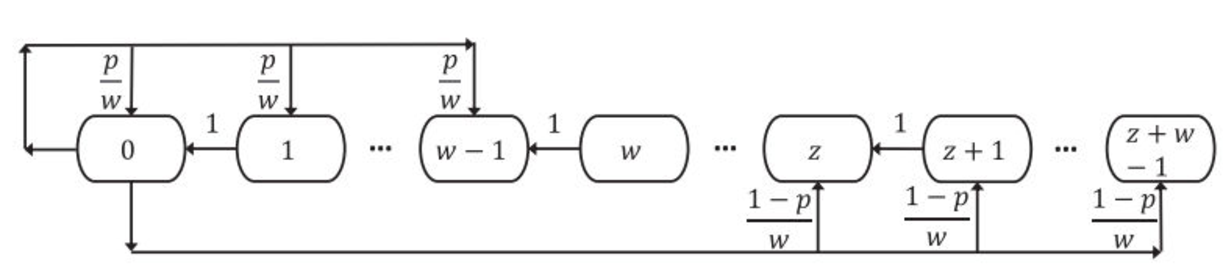
\includegraphics[width=0.8\textwidth]{figure/cp4/马尔可夫链.pdf}
\caption{目标节点的状态转移图}
\label{fig:cp4_mc_chain}
\end{figure}

我们将该一维马尔可夫链的平稳状态概率记为 $s_l$，其中状态空间 $l \in [0, z+w-1]$，具体演化过程如图\ref{fig:cp4_mc_chain}所示。记$T_{m,n}$为从状态$s_m$到$s_n$的转移概率。根据式\eqref{cp4_backoff_counter_evolution}，我们可以给出三种转移关系：
\begin{enumerate}[wide]
    \item 处于状态$s_0$的节点成功地发送一个包，之后它再$[z,z+w-1]$内随机选择了一个退避计时器，由于一个节点成功发送数据包的概率为 $1-p$，因此这个情况的转移概率为$\frac{1-p}{w}$。
    \item 处于状态$s_0$的节点发送的包与其他节点所发的包发生了碰撞，此时它将在$[0,w-1]$内随机选择一个退避计时器，由于一个节点碰撞的概率为 $p$，因此这个情况的转移概率为$\frac{p}{w}$.
    \item 节点不处于 $s_0$的状态，此时节点将会从$s_m$以1的概率转移到$s_{m-1}$。
\end{enumerate}
综上所述，我们可以对图\ref{fig:cp4_mc_chain}中的马尔可夫链所涉及的状态转移关系进行如下总结：
\begin{equation}\label{cp4_tmn}
    \begin{cases}
T_{0,n} = \frac{1-p}{w}, & \text{if } z \le n \le z + w - 1, \\
T_{0,n} = \frac{p}{w}, & \text{if } 0 \le n \le w - 1, \\
T_{m,m-1} = 1, & \text{if } m \neq 0.
\end{cases}
\end{equation}

\subsubsection{自洽方程的构建}
根据式\eqref{cp4_tmn}与图\ref{fig:cp4_mc_chain}的状态转移图，我们可以推导出：
\begin{enumerate}
    \item 当 $z\ge w$时，有
    \begin{equation}\label{cp4_zgew}
        s_l =
\begin{cases}
s_0 \left[ (1 - p) + \frac{p(w-l)}{w} \right], & \text{if } 0 \le l \le w - 1, \\
s_0 (1 - p), & \text{if } w \le l < z, \\
\frac{s_0 (1-p)(w+z-l)}{w}, & \text{if } z \le l \le z + w - 1.
\end{cases}
    \end{equation}
    \item 当 $z<w$时，有
    \begin{equation}\label{cp4_zlw}
        s_l =
\begin{cases}
s_0 \left[ (1 - p) + \dfrac{p(w-l)}{w} \right], & \text{if } 0 \le l \le z - 1, \\
s_0 \left[ \dfrac{(1-p)(z+w-l)}{w} + \dfrac{p(w-l)}{w} \right], & \text{if } z \le l < w, \\
\dfrac{s_0 (1-p)(z+w-l)}{w}, & \text{if } w \le l \le z + w - 1.
\end{cases}
    \end{equation}
\end{enumerate}

对于这两种情况，利用归一化条件 $\sum_{l=0}^{z+w-1}s_l$，代入式\eqref{cp4_zgew}或者式\eqref{cp4_zlw}，都可以得到以下结果：
\begin{equation}\label{cp4_s_0_and_p}
    s_0+z(1-p)s_0+\frac{s_0(w-1)}{2}=1
\end{equation}

为了求解出碰撞概率 $p$，我们需要找出 $s_0$ 与 $p$ 的关系。$s_0$ 是节点退避计时器处于0的状态，此时节点将发送包。在包含 $N$ 个活跃节点的竞争网络中，目标节点发生碰撞的充要条件是：在目标节点决定发送的同一时刻，剩余的 $N-1$ 个节点中至少有一个节点的退避计时器也恰好倒数至 0。因此，碰撞概率满足：
\begin{equation}\label{cp4_p_and_s0}
    p=1-(1-s_0)^{N-1}
\end{equation}
将式\eqref{cp4_p_and_s0}代入式\eqref{cp4_s_0_and_p}，可以将 $s_0$ 消去，得到只含 $p$ 的自洽方程 $f(p)=0$，即
\begin{equation}\label{cp4_ziqiafangcheng_p}
    [ 1 + z(1-p) + \frac{w-1}{2} ] ( 1 -\sqrt[N -1]{1-p} ) - 1=0
\end{equation}

\subsubsection{自洽方程解的存在唯一性论证}
为了利用数值迭代算法求解该方程，必须在理论上严格论证其在定义域 $(0, 1)$ 内稳态解的存在性与唯一性。

我们引入中间变量 $x=\sqrt[N-1]{1-p}$，由于真实的碰撞概率 $p$ 满足 $0<p<1$，因此 $0<x<1$，此时 $f(p)$ 可写作如下形式：
\begin{equation}\label{cp4_ziqiafangcheng_x}
    (zx^{N-1}+\frac{w+1}{2})(1-x)=1
\end{equation}

为了分析方程\eqref{cp4_ziqiafangcheng_x}解的特性，我们将该方程中的 $z$ 进行分离，可以得到：
\begin{equation}\label{cp4_ziqiafangcheng_z}
    z=\frac{2-(w+1)(1-x)}{2x^{N-1}(1-x)}
\end{equation}
将方程\eqref{cp4_ziqiafangcheng_z}的右边记为函数 $H(x)$，由于 $z>0$，因此必须满足 $2-(w+1)(1-x)>0$，即 $x>\frac{w-1}{w+1}$。

首先分析解的存在性，当 $x\to (\frac{w-1}{w+1})^+$时，$H(x)$的分子趋近于0且分母为正数，故 $H(x)\to 0$;当 $x\to 1^-$时，分母趋近于0且分子趋近于1，故 $H(x)\to +\infty$。由于 $H(x)$是一个连续的函数，根据介值定理，对于任意大于0的常数 $z$，必定存在至少一个 $x^*$，使得 $H(x^*)=z$。因此，方程的解必定存在。

接下来分析解的唯一性。对 $H(x)$ 进行求导，得到：
\begin{equation}
    H'(x) = \frac{x^{N-2}}{ [x^{N-1}(1-x)]^2 } \cdot Q(x)
\end{equation}
其中，$Q(x)$为一个二次函数，具体形式为：
\begin{equation}
    Q(x) = \frac{(w-1)(N-1)}{w+1}x^2 + [N - \frac{2(w-1)(N-1)}{w+1}]x - \frac{2(N-1)}{w+1}
\end{equation}
由于 $H'(x)$ 的最前面的分式大于0，因此函数 $H(x)$ 的单调性完全由 $Q(x)$ 决定。观察 $Q(x)$，其二次项系数大于0，因此 $Q(x)$ 是一条开口向上的抛物线，要使 $H'(x)>0$ 恒成立，即保证函数 $H(x)$ 单调递增，就必须保证 $Q(x)$ 与 $x$ 轴没有交点，那么就需要保证判别式 $\Delta<0$，计算判别式并进行化简，最终可得到：
\begin{equation}
    \Delta = N^2 - \frac{4(N-1)(w-1)}{w+1}<0
\end{equation}
对其进行整理，可以得到：
\begin{equation}\label{cp4_w}
    w>\frac{N^2-2N+2}{2(N-1)}>\frac{N-1}{2}
\end{equation}
由此我们得到了保证函数 $H(x)$ 单调递增的严格条件。

综上，当 $w$ 满足式\eqref{cp4_w}的条件时，我们能够保证方程\eqref{cp4_ziqiafangcheng_p}有唯一解，这确保我们能够使用数值迭代的方法来求解 $p$ 的具体数值。

\subsection{信息时效性指标的理论解析}
在确认了系统的稳态碰撞概率后，我们接下来着手求解等待 CSMA 网络下的平均 AoI 与 AoI 违规概率。尽管等待 CSMA 与等待 ALOHA 在底层退避机制与时隙结构上存在显著差异，但从宏观接收端的视角来看，数据包到达所引发的 AoI 演化轨迹依然呈现出高度相似的锯齿状特征。因此，第二章所推导的 AoI 通用计算框架在此依然严格适用。平均 AoI 可通过式\eqref{cp2_avg_aoi}降维后的式\eqref{cp3_avg_aoi}进行计算，AoI 违规概率则可沿用式\eqref{cp3_EJresult}中的矩匹配移位指数分布近似策略以及式\eqref{cp2_aoi_violation_expression}进行求解。因此我们的目标依旧是推导出连续两次成功传输间隔 $Y$ 的一阶矩 $E[Y]$ 与二阶矩 $E[Y^2]$。

与 ALOHA 机制中恒定的时隙长度不同，CSMA 网络中系统时隙的物理长度是随网络状态动态变化的。因此，在推导 $Y$ 时，我们必须将变长系统时隙这一因素也考虑进去。

\subsubsection{求解 Y 的一阶矩}
设两次成功的数据包传输之间的间隔 $Y$ 内一共发生了 $\alpha$ 次数据包的传输，之前我们假设了碰撞概率 $p$ 是一个常数，因此 $\alpha$ 服从参数为 $1-p$ 的几何分布，其概率质量函数为：
\begin{equation}\label{cp4_alpha}
    \text{Pr}\{\alpha=k\}=(1-p)*p^{k-1},k=1,2,\dots
\end{equation}

根据等待 CSMA 的设计规则，我们可以将一次完整的更新间隔 $Y$ 拆解成两个阶段。第一个阶段是节点在每次成功传输后，主动退避的 $z$ 个系统时隙，将这部分时隙长度记为 $U$。由于在这 $z$ 个系统时隙内，系统时隙的长度有 $p$ 的概率为1，也有 $1-p$ 的概率为$\frac{1}{M}$，因此 $U$ 的数学期望为：
\begin{equation}\label{cp4_EU}
    E[U] = z(p+\frac{1-p}{M})
\end{equation}

第二个阶段是节点在经历一次失败的传输，或者成功传输且刚刚退避完 $z$ 个系统时隙的时刻，从在 $[0,w-1]$ 内随机选择一个退避计时器 $\beta$，直至退避计时器归0且完成一次固定耗时的传输所经历的总时间，将这部分时间记为 $V$，则 $V$ 的期望为：

\begin{equation}\label{cp4_EV}
    E[V] = 1 + \sum_{\beta=0}^{w-1}\frac{\beta}{w}(p+\frac{1-p}{M})=1+\frac{w-1}{2}(p+\frac{1-p}{M})
\end{equation}

我们将已知两次成功传输之间共经历 $k$ 次传输尝试条件下的间隔时长记为 $Y_k$。根据等待 CSMA 的运行机制，我们可以得到 $Y_k = U + \sum_{j=1}^{k} V_j$。基于期望的线性可加性，其一阶矩为：
\begin{equation}\label{cp4_EYk}
    E[Y_k] = z \left( p + \frac{1-p}{M} \right) + k \left[ 1 + \frac{w-1}{2} \left( p + \frac{1-p}{M} \right) \right]
\end{equation}
联立式\eqref{cp4_alpha}和式\eqref{cp4_EYk},可以得到 $Y$ 的一阶矩
\begin{equation}
\begin{aligned}
E[Y] &= \sum_{k=1}^{\infty} \Pr\{\alpha = k\} \, E[Y_k] \\
&= z \left( p + \frac{1-p}{M} \right) \sum_{k=1}^{\infty} (1-p) p^{k-1} \\
&\quad + \left[ 1 + \frac{w-1}{2} \left( p + \frac{1-p}{M} \right) \right] \sum_{k=1}^{\infty} k (1-p) p^{k-1} \\
&= z \left( p + \frac{1-p}{M} \right) + \frac{1}{1-p} + \frac{\left( p + \frac{1-p}{M} \right) (w-1)}{2(1-p)}
\end{aligned}
\label{cp4_EY}
\end{equation}
上式中包含了几何分布的零阶矩与一阶矩的求和形式，即$\sum_{k=1}^{\infty}(1-p)p^{k-1}=1$与$\sum_{k=1}^{\infty}k(1-p)p^{k-1}=\frac{1}{1-p}$。

\subsubsection{求解 Y 的二阶矩}
为了后续书写的方便，记 $\phi=z(p+\frac{1-p}{M})$，$\gamma = \frac{(w-1)(p+\frac{1-p}{M})}{2}$。$U$ 的一阶矩已由式\eqref{cp4_EU}给出，接下来求解 $U$ 的二阶矩。在 $z$ 个时隙中，假设有 $i$ 个时隙发生了碰撞，剩余 $z-i$ 个时隙空闲。由于 $i$ 服从二项分布 $B(z, p)$，根据二项式定理及二项分布的高阶统计特性：
\begin{equation}
    E[U^2] = \sum_{i=0}^{z} \binom{z}{i} p^i (1-p)^{z-i} \left(i + \frac{z-i}{M}\right)^2
\end{equation}
展开平方项并利用一阶矩性质 $\sum i \binom{z}{i}p^i(1-p)^{z-i} = zp$ 与二阶矩性质 $\sum i^2 \binom{z}{i}p^i(1-p)^{z-i} = p^2(z^2-z) + zp$ 进行化简，可得：
\begin{equation}
    \begin{aligned}
        E[U^2] &= z^2\left(p + \frac{1-p}{M}\right)^2 + zp(1-p)\frac{(M-1)^2}{M^2} \\
               &= \phi^2 + zp(1-p)\frac{(M-1)^2}{M^2}
    \end{aligned}
\end{equation}

同理，对于单次竞争周期，在给定随机抽取的退避计时器为 $\beta$ 的条件下，$V_\beta$ 的二阶条件期望为：
\begin{equation}
    E[V_\beta^2] = \sum_{i=0}^{\beta} \binom{\beta}{i} p^i (1-p)^{\beta-i} \left(i + \frac{\beta-i}{M} + 1\right)^2
\end{equation}
化简可得：
\begin{equation}
    \begin{aligned}
        E[V_\beta^2] &= \beta^2\left(p + \frac{1-p}{M}\right)^2 + \beta p(1-p)\frac{(M-1)^2}{M^2} \\
                     &\quad + 2\beta\left(p + \frac{1-p}{M}\right) + 1
    \end{aligned}
\end{equation}

由于 $\beta$ 在 $[0, w-1]$ 上均匀分布，对 $\beta$ 取平均，得到无条件二阶矩：
\begin{equation}
    \begin{aligned}
        E[V^2] &= \frac{1}{w}\sum_{\beta=0}^{w-1} E[V_\beta^2] \\
               &= \frac{2\gamma^2(2w-1)}{3(w-1)} + \frac{(w-1)p(1-p)(M-1)^2}{2M^2} + 2\gamma + 1
    \end{aligned}
\end{equation}

在获取了 $U$ 和 $V$ 的特征后，我们采用递归法求解二阶矩 $E[Y_k^2]$。当 $k=1$ 时,
\begin{equation}\label{cp4_EY1^2}
    \begin{split}
E\left[Y_1^2\right] &= E\left[(U + V)^2\right] = E\left[U^2\right] + 2E\left[U\right]E\left[V\right] + E\left[V^2\right] \\
&= \phi^2 + zp(1 - p) \frac{(M - 1)^2}{M^2} + 2\phi(1 + \gamma) + E\left[V^2\right].
\end{split}
\end{equation}

对于任意 $k \ge 1$，由于 $Y_{k+1}=Y_k + V$，因此 $E[Y_{k+1}^2]=E[Y_k^2]+2E[Y_k]E[V]+E[V^2]$，做差可得：
\begin{equation}\label{cp4_EYK+1^2-EYk^2}
    \begin{split}
E\left[Y_{k+1}^2\right] - E\left[Y_k^2\right] &= 2E\left[Y_k\right]E\left[V\right] + E\left[V^2\right] \\
&= 2\phi(1 + \gamma) + 2k(1 + \gamma)^2 + E\left[V^2\right].
\end{split}
\end{equation}
通过级数累加求和，我们可以得到 $Y_k$ 的二阶矩：
\begin{equation}
    \begin{split}
E\left[Y_k^2\right] &= \phi^2 + zp(1 - p) \frac{(M - 1)^2}{M^2} + 2k\phi(1 + \gamma) \\
&\quad + k(k - 1)(1 + \gamma)^2 + kE\left[V^2\right].
\end{split}
\end{equation}

最后，我们得到 $Y$ 的二阶矩：
\begin{equation}
    \begin{split}
E\left[Y^2\right] &= \sum_{k=1}^{\infty} (1-p) p^{k-1} E\left[Y_k^2\right] \\
&= \phi^2 + z p (1-p) \frac{(M-1)^2}{M^2} + \frac{2\phi(1+\gamma)}{1-p} \\
&\quad + \frac{2p(1+\gamma)^2}{(1-p)^2} + \frac{E\left[V^2\right]}{1-p} \\
&= \left( \phi + \frac{1+\gamma}{1-p} \right)^2 + \frac{p(M-1)^2}{M^2} \left[ z(1-p) + \frac{w-1}{2} \right] \\
&\quad + \frac{p(1+\gamma)^2}{(1-p)^2} + \frac{\gamma^2 (w+1)}{3(w-1)(1-p)}.
\end{split}
\end{equation}

至此，通过将求得的一阶矩与二阶矩代回分别代回式\eqref{cp2_avg_aoi}、式\eqref{cp3_EJresult}与式\eqref{cp2_aoi_violation_expression}，我们就能成功得到等待 CSMA 下的平均 AoI 与 AoI 违规概率的计算闭式。

